\documentclass[11pt]{article}
\usepackage[margin=2cm]{geometry}
\usepackage{amsmath,amssymb,bm}
\usepackage{booktabs}
\usepackage{graphicx}
\usepackage{float}
\usepackage[hidelinks]{hyperref}

\title{MMA3001 Project:\textit{ A Reproducible Surrogate-Modelling Workflow for a Composite Beam Benchmark}}
\author{James Morton -- 33853967}
\date{Draft for technical review -- \today}

\begin{document}
\maketitle

\begin{abstract}
This project develops a reproducible workflow for learning a structural response model from finite-element analysis (FEA), correcting it with a small number of known reference observations, and checking its predictive performance on held-out cases. Because the future target is a curved composite leaf-spring landing gear for which no convenient exact solution is available, the methodology is first exercised on a straight, linearly width-tapered cantilever with an analytical small-deflection reference. A preliminary set of 50 layered-shell cases was available for review. A Gaussian-process (GP) model and quadratic response surface were fitted, then a sparse analytical discrepancy correction was assessed. The GP predicted held-out analytical compliance with 0.139\% mean absolute percentage error (MAPE); correction using five reference cases gave 0.150\% MAPE. The correction did not improve this run. The archived 100 N results have absolute deflections from 0.54 to 1.77 times beam length, outside the analytical model's small-deflection assumptions. These results therefore demonstrate the workflow only; they do not validate a physical material model or provide a final engineering prediction. A lower-load run, mesh study, and recorded solver provenance are required before drawing stronger conclusions.
\end{abstract}

\section{Problem definition and scope}
The engineering problem motivating the work is to reduce the cost of building response models for composite landing-gear geometry. Repeated physical testing can be expensive. The proposed future workflow is to generate an FEA response database, use a limited number of true observations to correct systematic model discrepancy, and predict responses at unobserved design points. This project does not include physical testing data. It studies whether the workflow can be implemented and tested against an analytical reference before application to curved landing gear.

The benchmark is a straight cantilever fixed at its root and loaded transversely at its free tip. The planform width decreases linearly from root width $b_0$ to tip width $r_b b_0$, where $r_b$ is the taper ratio. The laminate thickness and layup are held fixed. This benchmark is a methods test: it is not a geometric representation of an undercarriage and does not model impact, contact, damage, ply failure, material nonlinearity, or dynamic landing response. The project scope and proposal require coordinator approval under the course brief; record the approval decision here before final submission: \textbf{[student: enter approval status and date]}.

\section{Inputs, outputs, and design domain}
The fitted response is tip compliance $C=|\delta|/P$ in metres per newton. Fitting compliance makes sense for the linear elastic model because deflection scales with applied load. The design inputs varied in the archived dataset are beam length $L$, root width $b_0$, and taper ratio $r_b$. The load, material definition, ply sequence, thickness, supports, and mesh are fixed. The exact range of the 50 archived cases is shown in Table~\ref{tab:domain}. These observed ranges are a data domain, not certified engineering limits.

\begin{table}[H]
\centering
\caption{Inputs and observed design domain in the preliminary sweep.}
\label{tab:domain}
\begin{tabular}{llll}
\toprule
Input/output & Symbol & Units & Values / domain \\
\midrule
Beam length & $L$ & m & 0.4023--0.5978 \\
Root width & $b_0$ & m & 0.04017--0.05974 \\
Taper ratio & $r_b=b_{tip}/b_0$ & -- & 0.4053--0.8920 \\
Tip load & $P$ & N & 100 (fixed in archived run) \\
Layup thickness & $h$ & m & 0.00350 (fixed, 20 plies) \\
Tip deflection & $\delta$ & m & FEA output; signed in CSV \\
Compliance & $C=|\delta|/P$ & m/N & Fitting target \\
Laminate mass & $m$ & kg & FEA post-processing output \\
\bottomrule
\end{tabular}
\end{table}

The current fitting script requires finite values for all geometry and compliance columns, positive compliance, and at least 16 complete records. Geometry must also satisfy positive length and width and $0<r_b\le 1$ for the analytical function. The benchmark script uses SI units. The sweep's fixed laminate is ten 0$^\circ$ carbon twill plies and ten 0$^\circ$ glass plies, alternated through thickness. Cured ply thicknesses are 0.20 mm and 0.15 mm respectively, giving 3.50 mm total. The glass is assumed to be UD E-glass/epoxy. The material constants are representative placeholders rather than measured values; the source notes and assumptions are recorded in \texttt{layup.json} and the bibliography. The carbon fabric values are informed by a prepreg data sheet and generic carbon-fabric properties \cite{guritSE84LV,performanceCarbonGeneric}; the glass lamina values are representative published values \cite{glassUDLamina}. The alternating sequence is unsymmetric and may exhibit extension--bending coupling.

The scripts write CSV sweep data and prediction tables, JSON metrics, a serialized model artifact, and a LaTeX results table. MAPDL must be installed and licensed for solver runs. The fitting and plotting scripts operate on saved data and do not require MAPDL.

\section{Analytical benchmark}
For a small-deflection, linearly elastic beam with bending and Timoshenko shear deformation, tip compliance is evaluated as
\begin{align}
C(L,b_0,r_b) &= \int_0^L \left[\frac{(L-x)^2}{b(x)D_{eff}} + \frac{1}{\kappa b(x)S_{eff}}\right] \, dx,\\
b(x)&=b_0\left[1-(1-r_b)\frac{x}{L}\right].
\label{eq:compliance}
\end{align}
Here $D_{eff}$ is laminate bending rigidity per unit width (N m), $S_{eff}$ is transverse shear rigidity per unit width (N/m), and $\kappa=5/6$ is the assumed shear correction factor. The reference value is $\delta=P C$. In the implementation, a 64-point Gauss--Legendre rule evaluates the integral.

For the 0$^\circ$ laminate, the code assembles the Classical Lamination Theory $A$, $B$, and $D$ matrices from ply in-plane reduced stiffnesses, following standard laminate theory \cite{reddyMechanics}. It obtains effective bending rigidity by inverting the full $ABD$ matrix under zero membrane resultants and zero non-$x$ bending moments, retaining coupling for the unsymmetric stack. The approximate shear rigidity is $S_{xz}=\sum_k G_{xz,k}t_k$. These are explicit benchmark choices; the shear model and material properties should be treated as assumptions. The comparison tests agreement between FEA and this chosen reference implementation, not truth for a real composite.

\section{FEA and surrogate method}
The archived sweep contains 50 cases calculated with a structured SHELL181 model, 40 elements along the beam and 6 across the width (240 shell elements per case), with three through-thickness integration points per ply. SHELL181 supports layered sections defined through section data commands \cite{ansysShell181,pymapdlSections}. Each case represents a static linear solution with a 100 N transverse tip force. The root is clamped and the laminate section uses 20 explicit plies. The result archive does not contain the MAPDL release, PyMAPDL release, solver log, or a run manifest; the metrics label its origin as “PyMAPDL FEA (assumed)”. These omissions limit reproducibility and provenance.

The model inputs are standardized dimensional quantities $(L,b_0,r_b)$ and the output is $C$. A fixed random seed splits the observations into 37 training points and 13 held-out test points. A degree-two polynomial response surface with ridge regression is used as an alternative baseline. The GP uses a Mat\'ern $\nu=2.5$ covariance kernel with standardized predictors. For sparse correction, five reference points are randomly selected from training data only. A second GP fits the discrepancy
\begin{equation}
\Delta C(\mathbf{x})=C_{ref}(\mathbf{x})-C_{FEA}(\mathbf{x}),\qquad
\widehat C_{corr}(\mathbf{x})=\widehat C_{FEA}(\mathbf{x})+\widehat{\Delta C}(\mathbf{x}),
\end{equation}
where $\mathbf{x}=(L,b_0,r_b)$. The held-out cases are not used to fit the raw model or discrepancy model. The code also supports a mass-constrained design demonstration, but a final engineering optimum is not claimed because no validated response domain or design deflection requirement has yet been established.

\section{Results and validation}
Table~\ref{tab:surrogate-validation} compares the held-out models. The quadratic baseline reproduces the source FEA compliance with 0.977\% MAPE. The raw GP reaches 0.139\% MAPE versus the analytical reference. Applying the sparse analytical correction results in 0.150\% MAPE. The correction thus slightly worsens the MAPE for this run, although its maximum percentage error is also marginally lower (0.618\% versus 0.651\%). The raw GP was already close to the analytical reference, leaving little systematic discrepancy for five points to correct.

% Generated by src/fit_corrected_surrogate.py; do not edit by hand.
\begin{table}[htbp]
\centering
\caption{Held-out performance for the beam benchmark using FEA data. Compliance is $|\delta|/P$.}
\label{tab:surrogate-validation}
\begin{tabular}{lrrrr}
\toprule
Method & RMSE & MAE & $R^2$ & MAPE (\%) \\
\midrule
Quadratic response surface (against FEA) & 8.460e-05 & 5.455e-05 & 0.9983 & 0.977 \\
Raw GP surrogate (against analytical reference) & 1.960e-05 & 9.052e-06 & 0.9999 & 0.139 \\
Corrected GP (against analytical reference) & 1.891e-05 & 9.167e-06 & 0.9999 & 0.150 \\
\bottomrule
\end{tabular}
\end{table}


The comparison is an interpolation test within the sampled parameter region; it is not a demonstration of extrapolation capacity. It assesses the model pipeline against an analytical benchmark while both use linear elastic assumptions. The validation target is not independent physical observation. No physical test results are part of the project and no physical validation claim is made.

\begin{figure}[H]
\centering
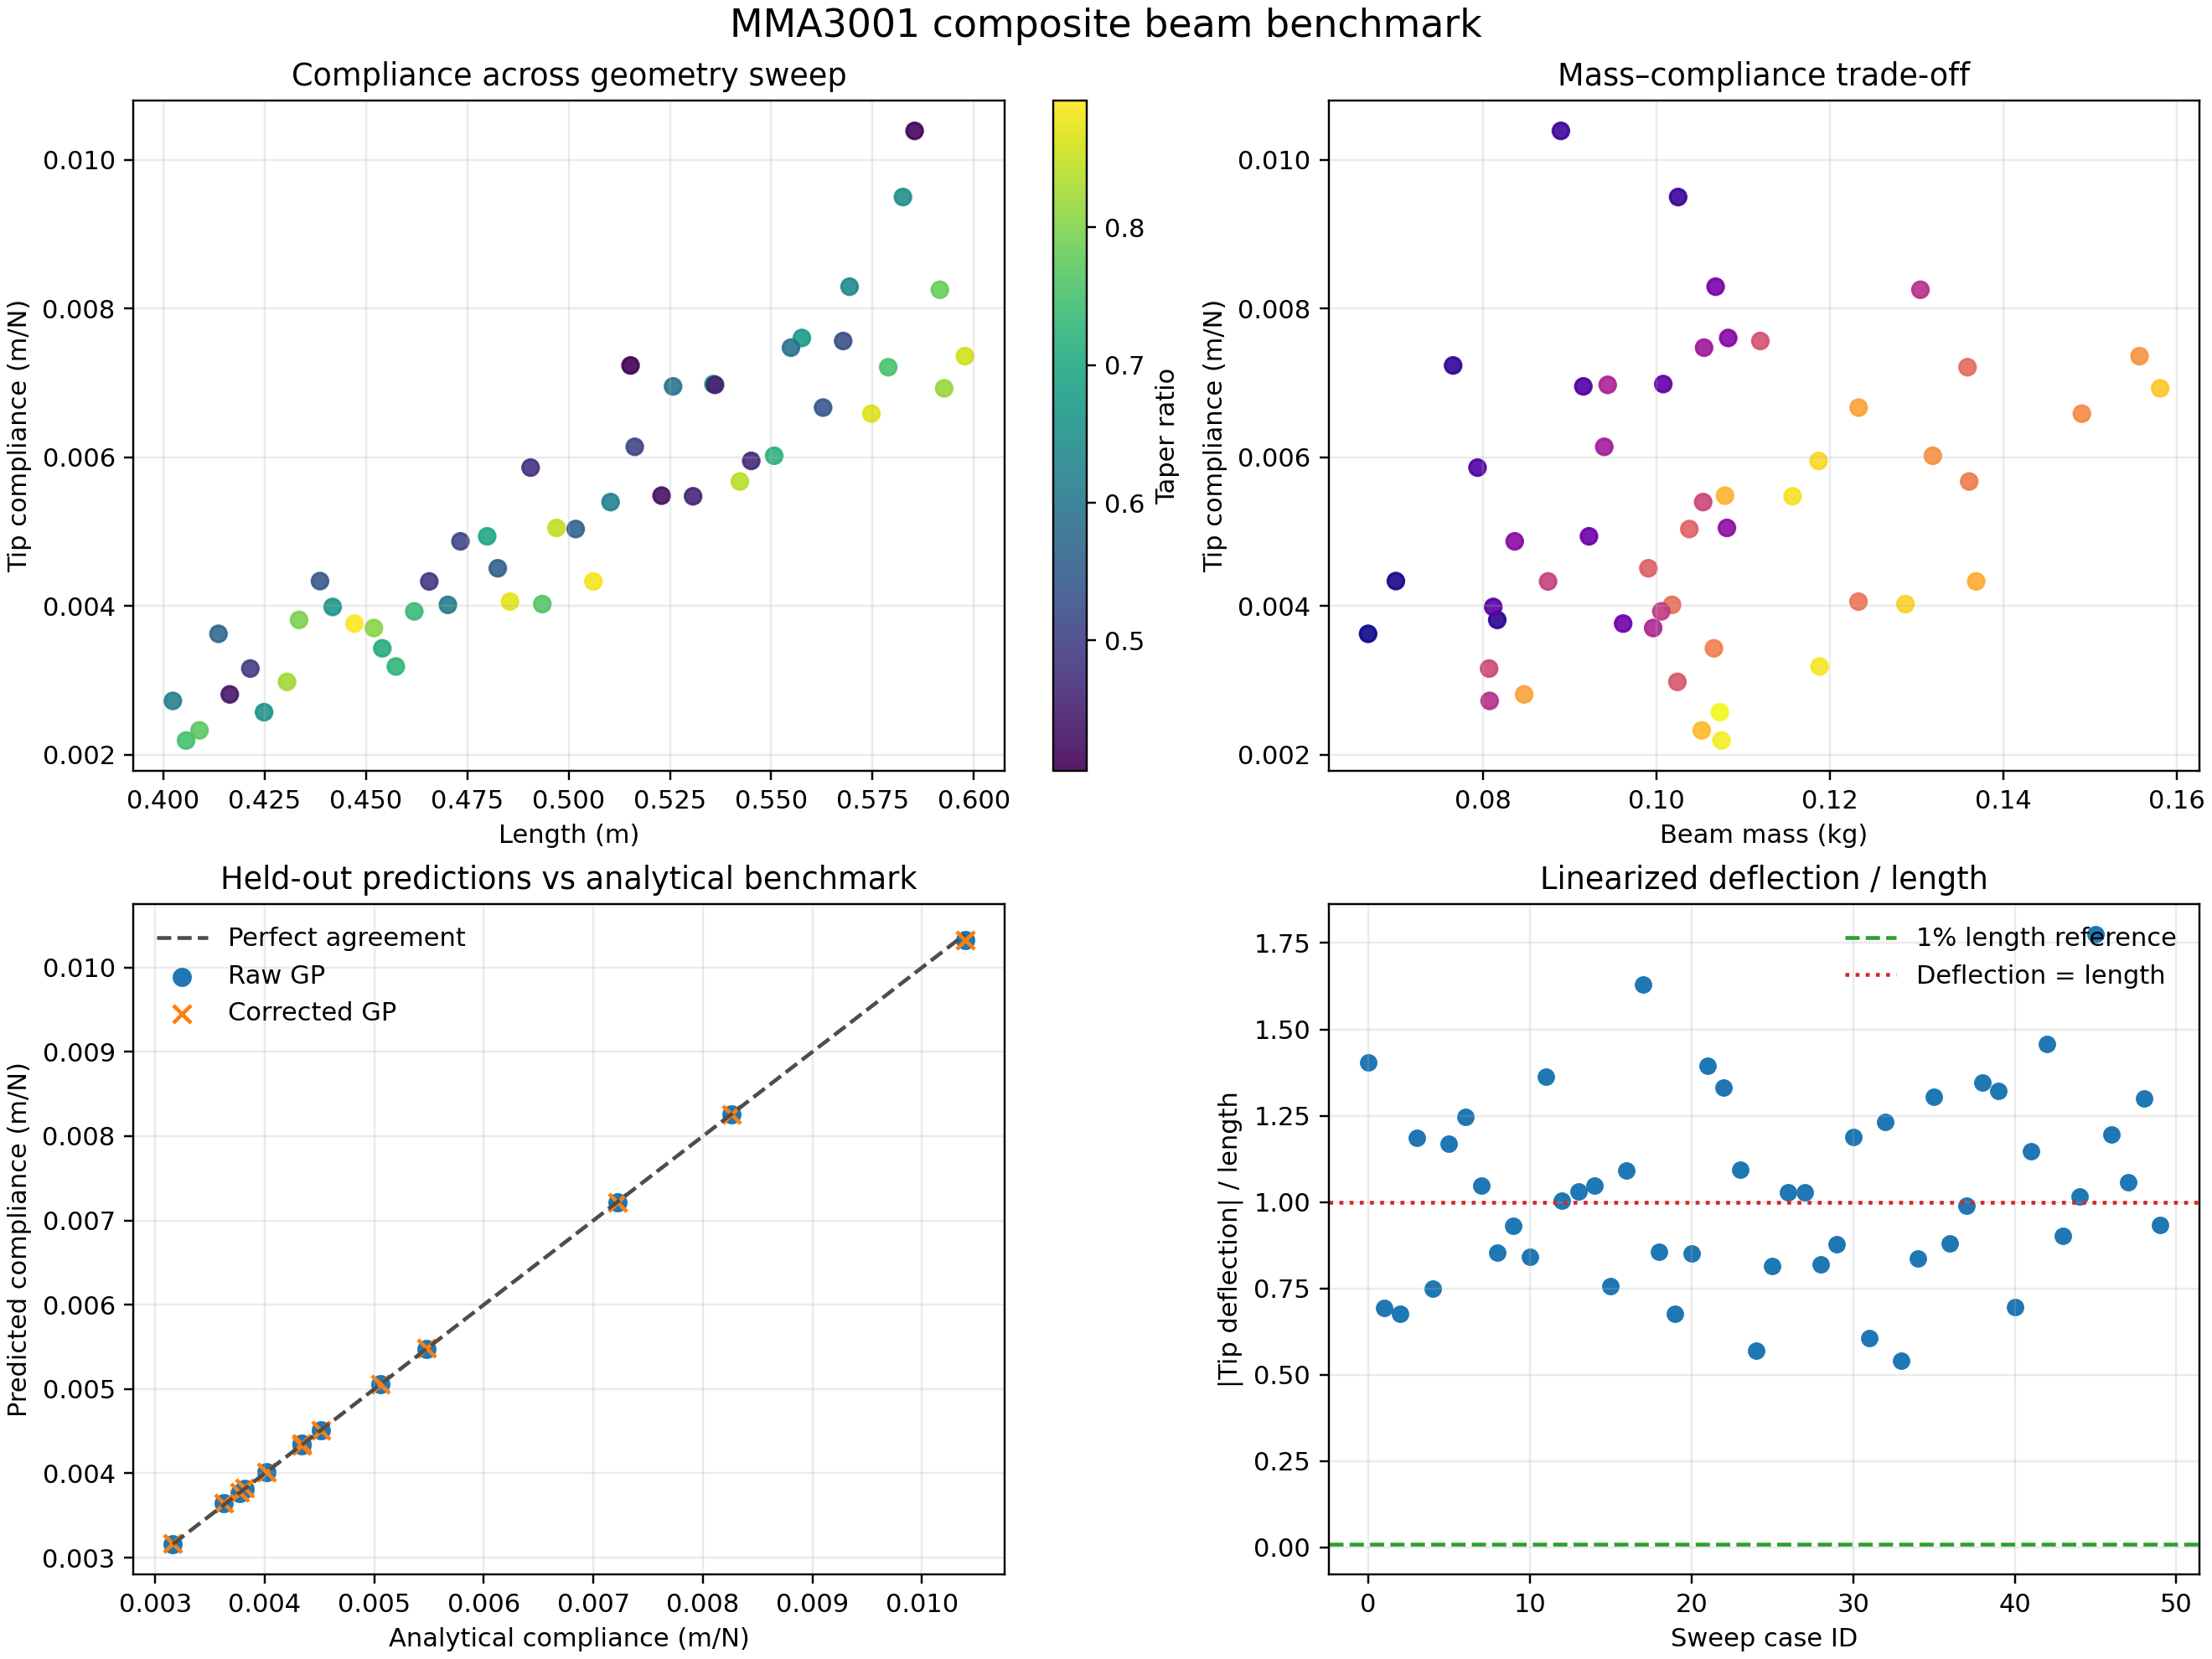
\includegraphics[width=0.88\linewidth]{../results/laminate_run_2026-10-17/figures/laminate_sweep_summary.png}
\caption{Summary of the archived preliminary sweep and held-out predictions. The large normalized deflections in the lower-right panel flag the small-deflection validity issue.}
\label{fig:sweep}
\end{figure}

\section{Validity, limitations, and next work}
The absolute deflection in the archived cases ranges from 0.219 m to 1.039 m for beam lengths from 0.402 m to 0.598 m; hence $|\delta|/L$ ranges from approximately 0.54 to 1.77. Those responses are far outside the small-deflection assumptions of Equation~\ref{eq:compliance}. The model should not be presented as an accurate small-deflection response at 100 N. The immediate next step is to re-run at a much lower load, confirm the load--deflection proportionality, and assess a suitably small $|\delta|/L$ domain.

The archive has only one mesh resolution, so mesh convergence remains untested. Re-run representative cases with progressively refined longitudinal and width divisions and report changes in compliance. Record MAPDL and PyMAPDL versions, solver output, element formulation and settings, boundary conditions, and run configuration. Review the shell local axes and material orientation, supports, force application, stress singularities, shear locking risk, and section behavior. Run the automated Python tests; they do not test a MAPDL solution. The material constants and density assumptions are not a calibrated or measured property set. The model omits geometric nonlinearity, contact, failure, impact, rate effects, and dynamic landing behavior.

Once the benchmark response is valid, evaluate interpolation using a fixed held-out design set and metrics such as RMSE, MAE, $R^2$, MAPE, and maximum relative error. Test extrapolation separately using a spatially separated region beyond the training envelope. Compare the quadratic baseline and GP, and repeat the split or use cross-validation to assess sensitivity to the small dataset. Report runtime for FEA, fitting, and prediction using a stated machine and software version; no timing evidence is currently present. A mass-optimal configuration can then be solved subject to a supplied deflection requirement, geometric bounds, and manufacturability constraints. Extending to a curved gear requires a new geometry parameterization and renewed validation; benchmark performance does not transfer automatically.

\section{Brief alignment and project deliverables}
The repository includes the functional source scripts, example inputs, results, unit-aware problem definition, a license, tests, test evidence, HTML API documentation, and this report draft. A requirement-by-requirement status and outstanding actions are listed in \texttt{docs/requirements\_traceability.md}. The project brief also requires a short presentation; it should present the problem, method, results, validation limits, alternatives, performance evidence, GitHub repository, and AI disclosure. Before submission, ensure the final compiled report is within the 5--10 page limit and replace all explicit student action notes with reviewed, supported information.

\section{AI use and student reflection}
AI tools were used to assist with drafting and editing project code, generating documentation scaffolding, identifying relevant material-property sources, debugging, and presenting analysis and plots. The student remains responsible for checking the code, the analytical derivation, source applicability, units, solver setup, and all reported values. Generated text or code is not evidence of correctness.

\textbf{Student reflection required:} \emph{[Add a concise first-person reflection describing the AI assistance actually used, one useful contribution, one limitation or error caught during review, how outputs were verified, and what decisions remained the student's own. Do not submit this placeholder unchanged.]}

\begin{thebibliography}{9}
\bibitem{guritSE84LV} Gurit, \emph{SE84LV High Performance Prepreg System: Product Data Sheet}, 2024. Available at \url{https://www.revchem.com/document/15pc135966a_tds-pdf/}.
\bibitem{performanceCarbonGeneric} Performance Composites, \emph{Mechanical Properties of Carbon Fibre Composite Materials}. Available at \url{https://performance-composites.com/carbonfibre/mechanicalproperties_2.asp}.
\bibitem{glassUDLamina} University of South Florida, \emph{Hooke's Law for a Two-Dimensional Unidirectional Lamina: Worked Example}. Available at \url{https://kaw.eng.usf.edu/compositesOCW/WorkedOutExamples/Section%202.4%20Hooke's%20Law%20for%20a%20Two%20Dimensional%20Unidirectional%20Lamina/Section2_4_worked_out_example_PPT/Section2_4_worked_out_example_PPT.html}.
\bibitem{reddyMechanics} J. N. Reddy, \emph{Mechanics of Laminated Composite Plates and Shells: Theory and Analysis}, 2nd ed., CRC Press, 2004.
\bibitem{ansysShell181} Ansys, Inc., \emph{SHELL181 Element Documentation}. Available at \url{https://ansyshelp.ansys.com/public/account/secured?returnurl=/Views/Secured/corp/v242/en/ans_elem/Hlp_E_SHELL181.html}.
\bibitem{pymapdlSections} Ansys, Inc., \emph{PyMAPDL secdata API}. Available at \url{https://mapdl.docs.pyansys.com/version/stable/api/_autosummary/ansys.mapdl.core.Mapdl.secdata.html}.
\end{thebibliography}
\end{document}
